% **************************** Define Graphics Path **************************
\ifpdf
\graphicspath{{Chapter3/Figs/Raster/}{Chapter3/Figs/PDF/}{Chapter3/Figs/}{Chapter3/Figs/Web/}{Chapter3/Figs/Server/}{Chapter3/Figs/Mobile/}}
\else
\graphicspath{{Chapter3/Figs/Vector/}{Chapter3/Figs/}}
\fi

\chapter{Thiết kế và Hiện thực}
\section{Thiết kế hệ thống}
\subsection{Kiến trúc mô hình hệ thống}
Như đã giới thiệu một số mô hình IoT thực tế ở Mục \ref{sec:xuhuongiot}, mô hình IoT phù hợp mà nhóm sẽ áp dụng cho việc pháp triển hệ thống giám sát được trình bày như Hình \ref{fig:pic5}. Hệ thống bao gồm các thành phần chính như sau: các node cảm biến, trung tâm lưu trữ dữ liệu và ứng dụng truy xuất và hiển thị thông tin phân tích dữ liệu.

\begin{figure}[H]
	\centering    
	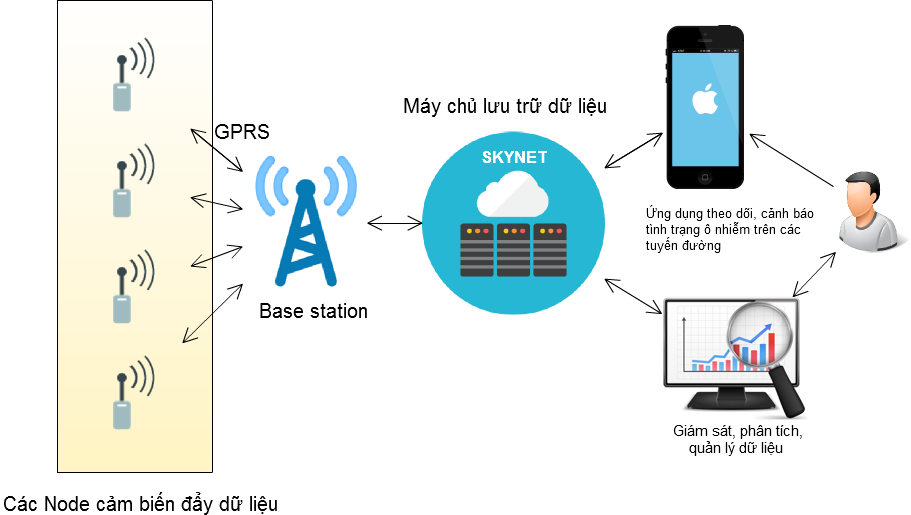
\includegraphics[width=1\textwidth]{system}
	\caption[Kiến trúc mô hình hệ thống]{Kiến trúc mô hình hệ thống}
	\label{fig:system}
\end{figure}

\newpage

\subsection{Các node cảm biến}
Các node cảm biến: là một thiết bị được lắp đặt trên những đoạn đường hoặc các địa điểm thích hợp cần để lấy dữ liệu tại khu vực đó, nhiệm vụ chủ yếu là lấy dữ liệu từ các cảm biến đo được sau đó gửi dữ liệu đó lên máy chủ bằng module Sim GPRS.
Để các node cảm biến này được hoạt động dưới tác nhân của môi trường như gió, mưa, bụi, và hơn hết có thể tận dụng nguồn năng lượng mặt trời để nạp pin cho mạch hoạt động độc lập với điện lưới, chúng tôi đã đề xuất mô hình thiết kế node cảm biến để có thể đáp ứng các yêu cầu như sau:
 
\begin{wrapfigure}{l}[4pt]{0.4\linewidth}
    
\includegraphics[scale=0.3]{house_home}
    \caption[Mô hình căn nhà 3D]{Mô hình căn nhà 3D}
    \label{fig:house_home}
\end{wrapfigure}
Lấy ý tưởng từ căn nhà gồm 4 bức tường và 2 mái che như Hình \ref{fig:house_home}, tấm năng lượng mặt trời được thiết kế và gắn như mái che của căn nhà, còn các mạch điện và cảm biến sẽ được đặt bên trong ngôi nhà xung quanh các bức tường được làm từ nhựa mica. Việc lắp đặt node cảm biến này theo hướng các tắm năng lượng mặt trời 1 phía hướng về đông và 1 phía hướng về tây nhằm giúp tắm năng lượng có thể lấy được năng lượng tối đa.

Từ kết quả tìm hiểu các loại khí thải trong mục \ref{sec:yeuto_khithai} đã được nên kết hợp với tình trạng các loại cảm biến hiện có trên thị trường hiện này thì nhóm chúng tôi đã quyết định đưa ra các loại cảm biến cần thiết cho một node cảm biến như sau:



%\\\\\\\\\\\\\\\\\\\\\\\\\\\\\\\\\\\\\\GP2\\\\\\\\\\\\\\\\\\\\\\\\\\\\\\\\\\\\\\\\\\\\%
\subsubsection*{Cảm biến bụi GP2} 
Cảm biến bụi GP2 là một bộ cảm biến chất lượng không khí quang học, được thiết kế đo những hạt bụi. Cám biến được thiết kế một điốt phát hồng ngoại và một photostransistor được sắp xếp thành đường chéo thiết bị này, cho phép nó phát hiện ánh sáng phản xạ của bụi trong không khí.  Nó đặc biệt hiệu quả trong việc phát hiện các hạt rất mịn như khói thuốc lá, và thường được sử dụng trong các hệ thống lọc không khí.

Cảm biến bụi GP2 tiêu tốn dòng rất ít (20 mA cao nhất, 11mA chế độ chạy thường), có thể hỗ trợ nguồn cung cấp lên tới 7VDC. Tín hiệu đầu ra của cảm biến là dạng tín hiệu tương tự dùng để đo mật độ bụi, với độ nhạy $0.5V/0.1mg/{m}^{3}$.

Thông số kỹ thuật:
\begin{itemize}
\item[•]Nguồn hoạt động: 5VDC
\item[•]Dòng tiêu thụ: 10mA
\item[•]Ngõ ra analog
\item[•]Nhiệt độ hoạt động: $-40^{o}$ $-$ $85 ^{o}$ C
\end{itemize}

\begin{figure}[H]
	\centering    
	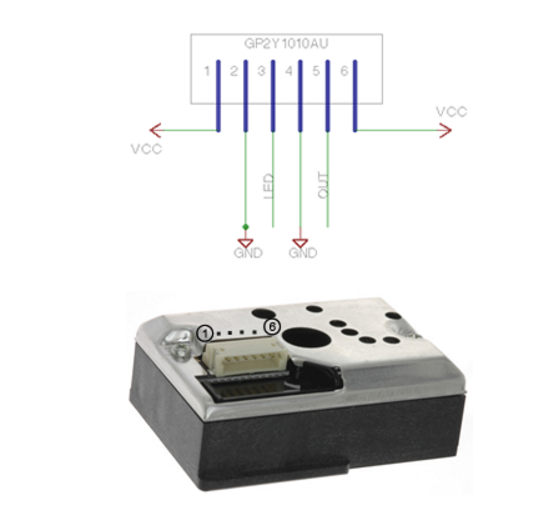
\includegraphics[width=0.5\textwidth]{gp2}
	\caption[Cảm biến bụi GP2 ]{Cảm biến bụi GP2}
	\label{fig:gp2}
\end{figure}

Sơ đồ kết nối cảm biến bụi GP2 với Arduino
Theo hướng dẫn của tài liệu kỹ thuật, nó có tất cả gồm 6 chân đầu ra để kết nối tới thiết bị. Để có thể cảm biến bụi GP2 hoạt động với vi xử lý Arduino cần kết nối như sơ đồ luận lý sau:

\begin{figure}[H]
	\centering    
	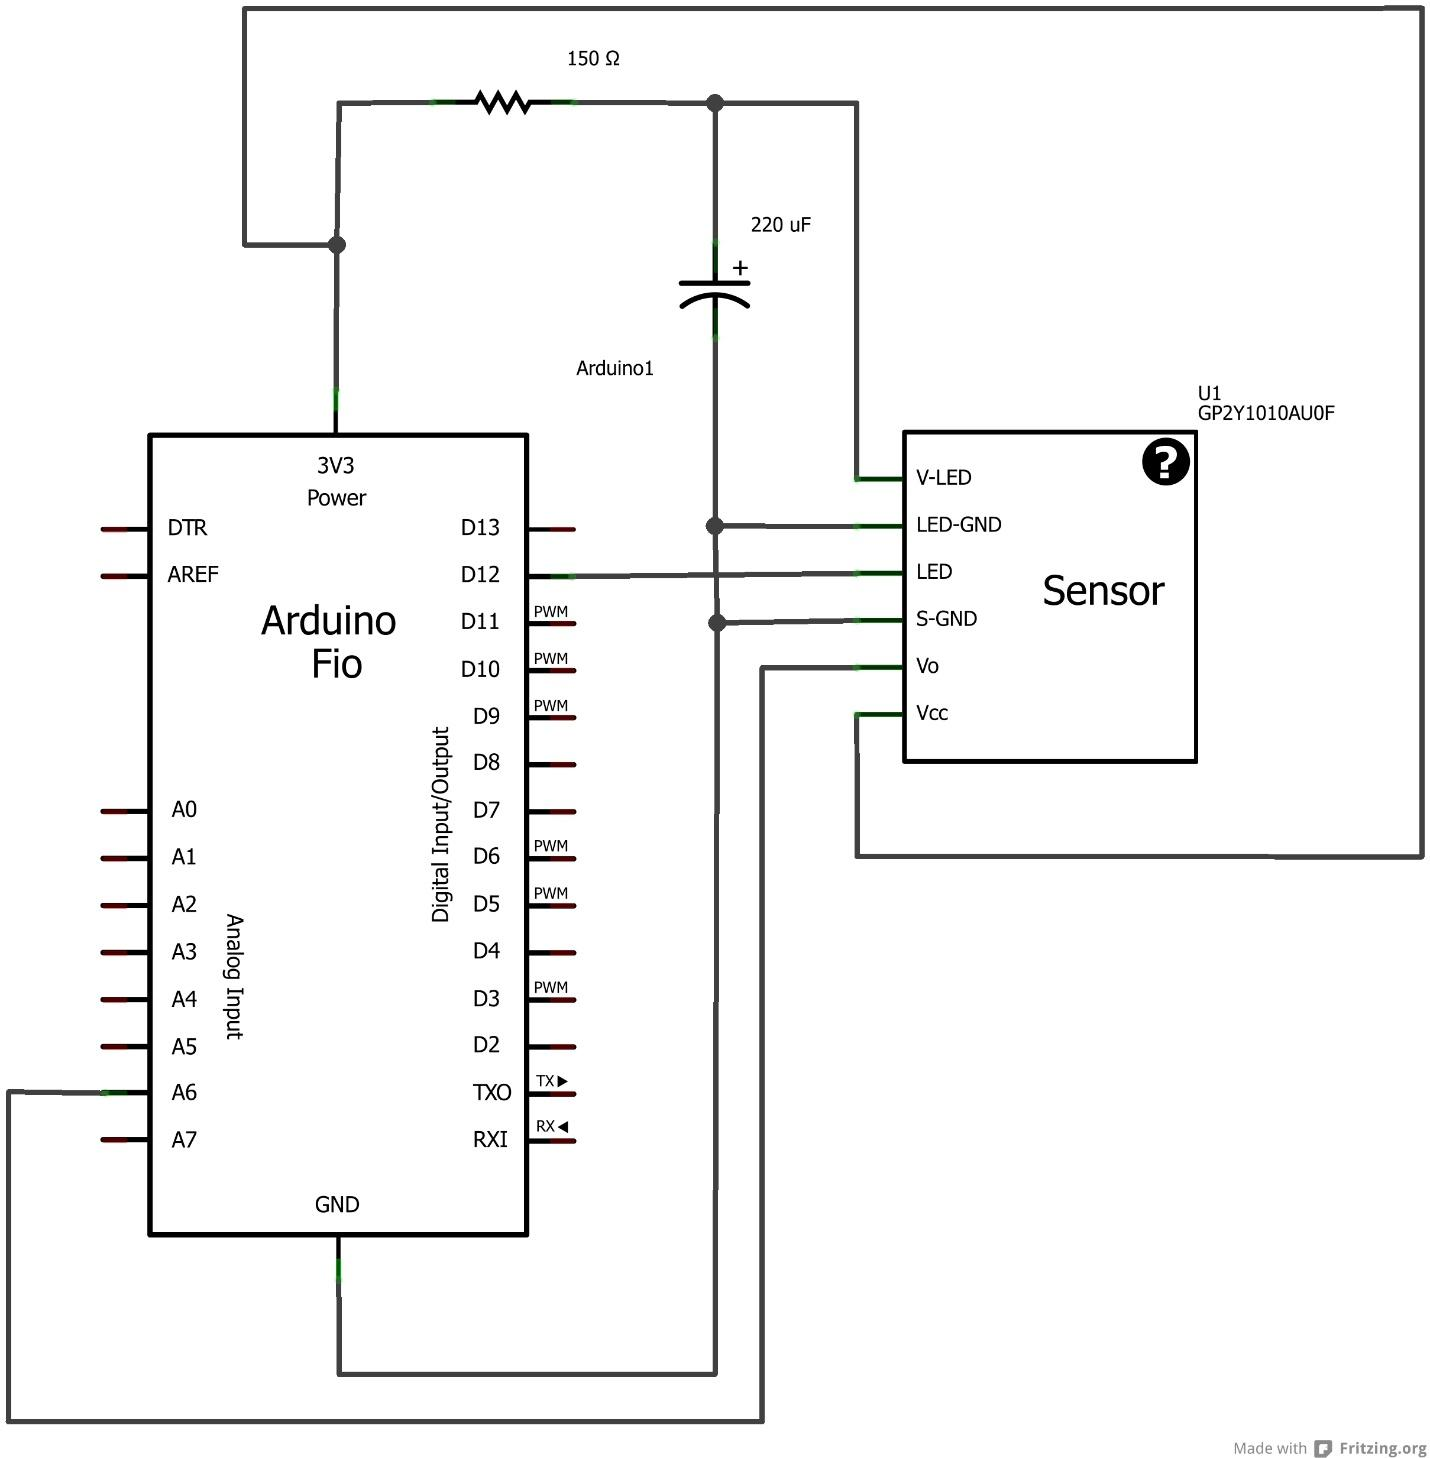
\includegraphics[width=0.7\textwidth]{sodogp2}
	\caption[Sơ đồ GP2 kết nối với Arduino ]{Sơ đồ GP2 kết nối với Arduino}
	\label{fig:sodogp2}
\end{figure}






%\\\\\\\\\\\\\\\\\\\\\\\\\\\\\\\\\\\\\\	MQ135	\\\\\\\\\\\\\\\\\\\\\\\\\\\\\\\\\\\\\\\\\\\\%
\newpage
\subsubsection*{Cảm biến chất lượng không khí MQ135} 
Cảm biến chất lượng không khí MQ135 thường được dùng trong các thiết bị kiểm tra chất lượng không khí bên trong cao ốc, văn phòng, thích hợp để phát hiện khí NH3, Nox, Ancol, Benzen, khói và khí CO2.Cám biến này với độ nhạy cao và thời gian đáp ứng nhanh. Tín hiệu ngõ ra dạng analog và digital. Cảm biến này có thể hoạt động ở nhiệt độ từ khoảng: $-10^{o}$C đến $50^{o}$C và tiêu thụ dòng khoảng 300mA tại 5V.
\begin{figure}[H]
	\centering    
	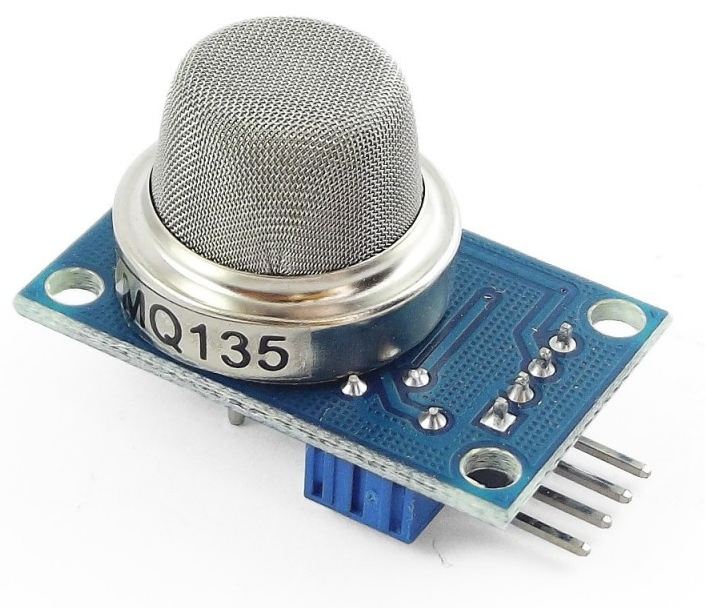
\includegraphics[width=0.7\textwidth]{mq135}
	\caption[Cảm biến MQ135]{Cảm biến MQ135}
	\label{fig:mq135}
\end{figure}
Thông số kỹ thuật:
\begin{itemize}
\item[•]Điện áp cung cấp: <=24 VDC
\item[•]Điện áp heater: 5V AC/DC
\item[•]Sử dụng chip so sánh LM393c.
\item[•]Hai tín hiệu đầu ra (digital và analog)
\item[•]Tín hiệu analog từ 0 ~ 5V.
\item[•]Dải phát hiện từ 10 đến 1000ppm
\end{itemize}

\begin{figure}[H]
	\centering    
	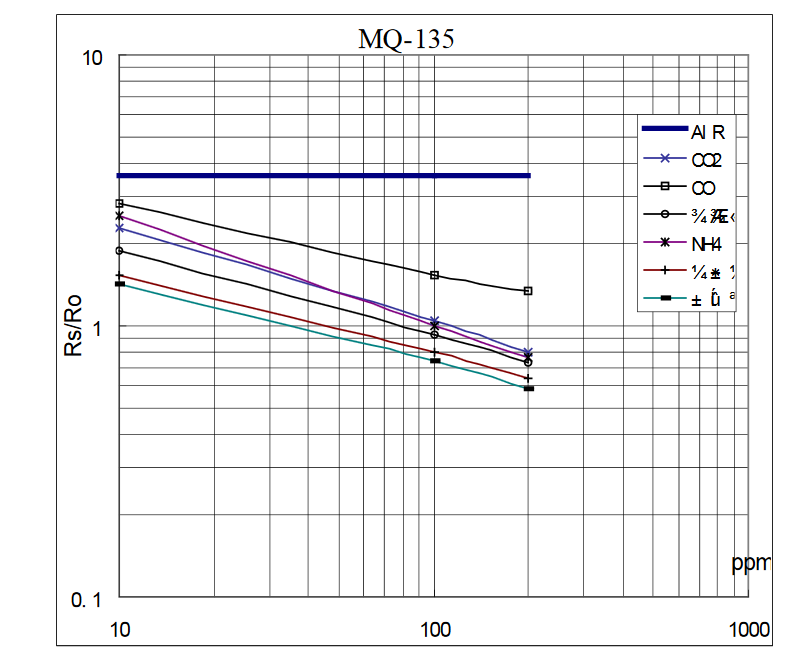
\includegraphics[width=0.7\textwidth]{mq135_mqh1}
	\caption[Giản đồ chỉ sự biến đổi của Rs/Ro và giá trị ppm của MQ135]{Giản đồ chỉ sự biến đổi của Rs/Ro và giá trị ppm của MQ135}
	\label{fig:mq135_mqh1}
\end{figure}

\begin{figure}[H]
	\centering    
	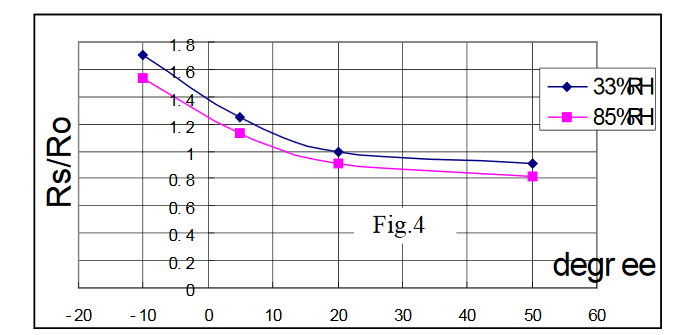
\includegraphics[width=0.7\textwidth]{mq135_mqh2}
	\caption[Giản đồ chỉ sự biến đổi của Rs/Ro đối với nhiệt độ, độ ẩm]{Giản đồ chỉ sự biến đổi của Rs/Ro đối với nhiệt độ, độ ẩm}
	\label{fig:mq135_mqh2}
\end{figure}


Giá trị chất lượng không khí(ppm) được xác định theo biểu đồ Hình \ref{fig:mq135_mqh1} giá trị này thay đổi theo sự biến đổi của giá trị Rs/Ro, theo Hình \ref{fig:mq135_mqh2} thì giá trị Rs/Ro bị ảnh hưởng bởi nhiệt độ và độ ẩm.

Để xác định được giá trị Rs/Ro từ ngõ ra analog của mạch cảm biến MQ-135 ta có công thức như sau:
\begin{center}
$\displaystyle \frac{R_{S}}{R_{L}} = \frac{V_{C}-V_{RL}}{V_{RL}}$
\end{center}

Giá trị Rs/Ro này được vi xử lý tính toán dựa trên đầu ra analog của cảm biến MQ-135 và được đưa vào thư viện mq135.h để có thể lấy được giá trị chất lượng không khí ppm theo sự thay đổi của nhiệt độ và độ ẩm của môi trường thực tế.

Thư viện mq135.h cung cấp cho chúng ta các hàm toán học đã được nhà sản xuất tính toán sẵn để có thể lấy được giá trị chất lượng không khí ppm dựa vào thay đổi của môi trường nhiệt độ và độ ẩm.



%\\\\\\\\\\\\\\\\\\\\\\\\\\\\\\\\\\\\\\	MQ07	\\\\\\\\\\\\\\\\\\\\\\\\\\\\\\\\\\\\\\\\\\\\%
\newpage
\subsubsection*{Cảm biến chất lượng không khí MQ07} 
Cảm biến khí CO MQ-7 có thể pháp hiện khí CO tập trung ở những nơi khác nhau từ 10 đến 1000ppm. Cám biến này với độ nhạy cao và thời gian đáp ứng nhanh. Tín hiệu ngõ ra dạng analog và digital. Cảm biến này có thể hoạt động ở nhiệt độ từ khoảng: -10C đến 50C và tiêu thụ dòng khoảng 250mA tại 5V.
\begin{figure}[H]
\centering    
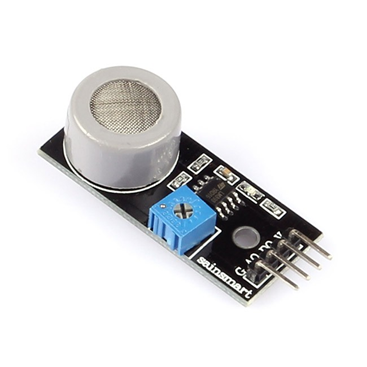
\includegraphics[width=0.7\textwidth]{mq07}
\caption[Cảm biến MQ07]{Cảm biến MQ07}
\label{fig:mq07}
\end{figure}


Thông số kỹ thuật:
\begin{itemize}
\item[•]Điện áp cung cấp: 3 ~ 5VDC.
\item[•]Sử dụng chip so sánh LM393 và MQ-7.
\item[•]Hai tín hiệu đầu ra (digital và analog)
\item[•]Tín hiệu analog từ 0 ~ 5V.
\item[•]Dải phát hiện từ 10 đến 1000ppm
\item[•]Kích thước: 33 x 20 x 16mm.
\end{itemize}
\begin{figure}[H]
\centering    
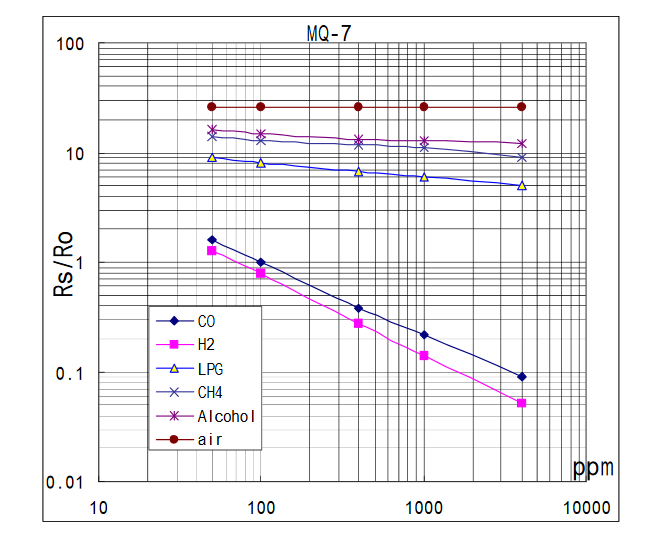
\includegraphics[width=0.7\textwidth]{mq07_mqh1}
\caption[Giản đồ chỉ sự biến đổi của Rs/Ro và giá trị ppm của MQ07]{Giản đồ chỉ sự biến đổi của Rs/Ro và giá trị ppm của MQ07}
\label{fig:mq07_mqh1}
\end{figure}


\begin{figure}[H]
\centering    
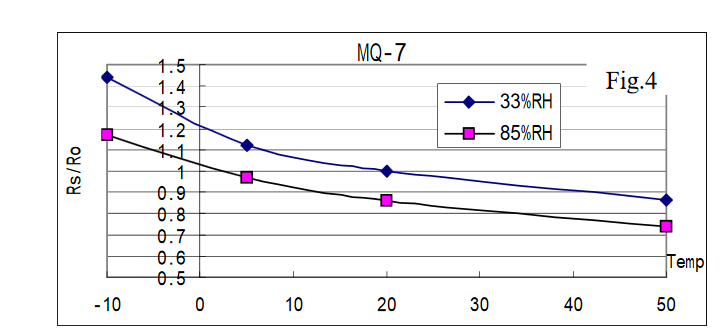
\includegraphics[width=0.7\textwidth]{mq07_mqh2}
\caption[Giản đồ chỉ sự biến đổi của Rs/Ro đối với nhiệt độ, độ ẩm]{Giản đồ chỉ sự biến đổi của Rs/Ro đối với nhiệt độ, độ ẩm}
\label{fig:mq07_mqh2}
\end{figure}


Giá trị chất lượng không khí(ppm) được xác định theo biểu đồ Hình \ref{fig:mq07_mqh1} giá trị này thay đổi theo sự biến đổi của giá trị Rs/Ro, theo Hình \ref{fig:mq07_mqh2} thì giá trị Rs/Ro bị ảnh hưởng bởi nhiệt độ và độ ẩm.

Để xác định được giá trị Rs/Ro từ ngõ ra analog của mạch cảm biến MQ-7 ta có công thức như sau:
\begin{center}
$\displaystyle \frac{R_{S}}{R_{L}} = \frac{V_{C}-V_{RL}}{V_{RL}}$
\end{center}

Giá trị Rs/Ro này được vi xử lý tính toán dựa trên đầu ra analog của cảm biến MQ-7 và được đưa vào thư viện mq07.h để có thể lấy được giá trị chất lượng không khí ppm theo sự thay đổi của nhiệt độ và độ ẩm của môi trường thực tế.

Thư viện mq07.h cung cấp cho chúng ta các hàm toán học đã được nhà sản xuất tính toán sẵn để có thể lấy được giá trị chất lượng không khí ppm dựa vào thay đổi của môi trường nhiệt độ và độ ẩm.






%\\\\\\\\\\\\\\\\\\\\\\\\\\\\\\\\\\\\\\	Cảm biến nhiệt độ DS18B20 IC	\\\\\\\\\\\\\\\\\\\\\\\\\\\\\\\\\\\\\\\\\\\\%
\newpage
\subsubsection*{Cảm biến nhiệt độ DS18B20 IC} 
Cảm biến nhiệt độ DS18B20 là cảm biến loại tín hiệu đầu ra digital đo nhiệt độ mới của hãng MAXIM với độ phân giải cao (12bit). IC được sử dụng giao tiếp 1 dây rất gọn gàng, dễ lập trình và giao tiếp nhiều DS18B20 trên cùng 1 dây. IC còn có chức năng cảnh báo nhiệt độ khi vượt ngưỡng và đặc biệt hơn là có thể cấp nguốn từ chân data.

\begin{figure}[H]
	\centering    
	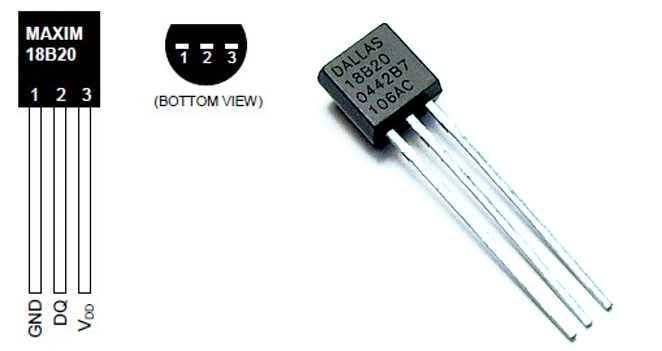
\includegraphics[width=0.7\textwidth]{ds18b20}
	\caption[Cảm biến nhiệt độ DS18B20]{Cảm biến nhiệt độ DS18B20}
	\label{fig:ds18b20}
\end{figure}

Thông số kỹ thuật:
\begin{itemize}
\item[•]Nguồn: 3-5.5V
\item[•]Dải đo nhiệt độ: -55 -125 * C
\item[•]Sai số: +-0.5 *C
\item[•]Độ phân giải: 9-12bits
\item[•]Thời gian chuyển đổi nhiệt độ: 750ms
\end{itemize}
Sơ đồ kết nối IC BS18B20 để lấy được tín hiệu data
\begin{figure}[H]
	\centering    
	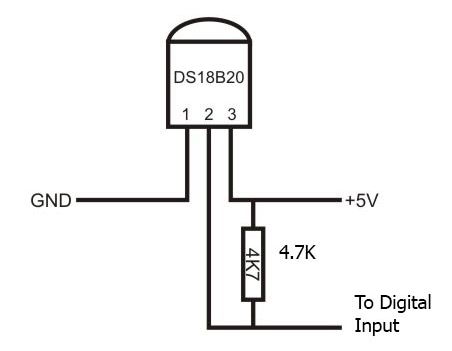
\includegraphics[width=0.7\textwidth]{ds18b20_ketnoi}
	\caption[Sơ đồ kết nối DS18B20]{Sơ đồ kết nối DS18B20}
	\label{fig: ds18b20_ketnoi}
\end{figure}
Chân Digital input sẽ được đưa tới chân Digital input của board arduino nano, hiện tại nhà sản xuất cũng cung cấp cho lập trình viên về bộ thư viện để có thể sử dụng trong việc phát triển.

\newpage







































\subsection{Chuẩn giao tiếp giữa các node tới máy chủ}
Để các node cảm biến gửi dữ liệu lên máy chủ thì chúng tôi đã sử dụng module Sim800L được giới thiệu trong mục \ref{sec:sim800l}. Quá trình kết nối của các node cảm biến tới máy chủ thông qua giao thức TCP được thực hiện dựa trên mô hình máy trạng thái như sau:


\begin{figure}[H]
\centering   
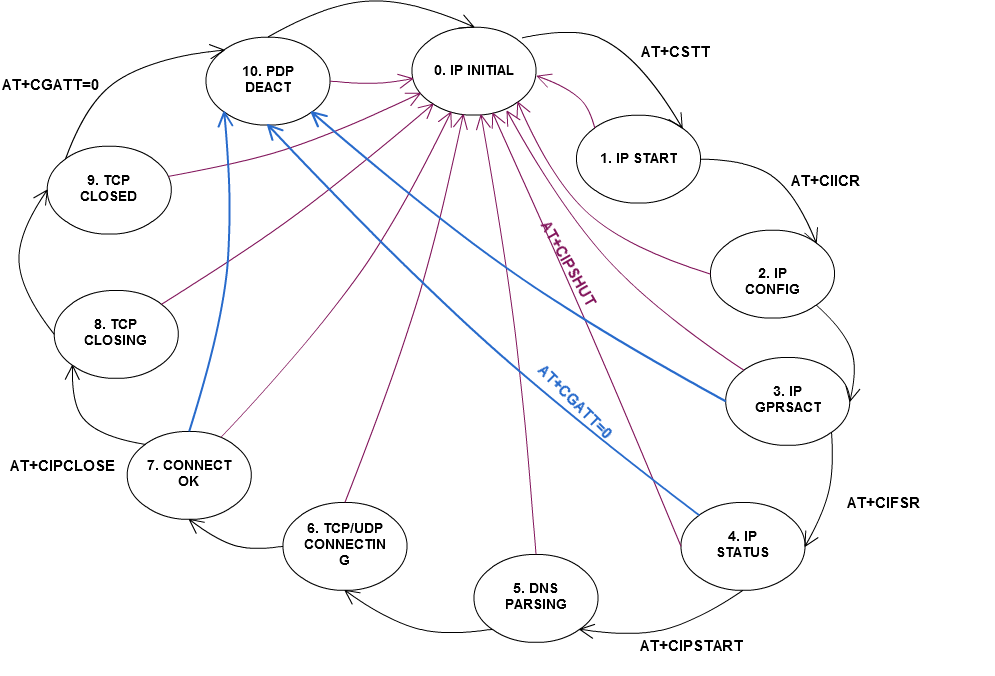
\includegraphics[width=1\textwidth]{sim800_status}
\caption[Sơ đồ trạng thái GPRS cho đơn kết nối]{Sơ đồ trạng thái GPRS cho đơn kết nối}
\label{fig:sim800_status}
\end{figure}

Để gửi được dữ liệu đến máy chủ cần phải thiết lập được kết nối TCP từ module SIM800 đến máy chủ thông qua 11 trạng thái như Hình \ref{fig:sim800_status}, các trạng thái được chuyển đổi thông qua các tập lệnh AT đã được đề cập tại mục \ref{sec:sim800l}. Đến trạng thái 7 (CONNET OK) chúng ta đã giữ được kết nối TCP tới máy chủ và tại trạng thái này dùng lệnh AT+CIPSEND để thực hiện việc gửi gói dữ liệu lên cho máy chủ.

Gói dữ liệu được gửi theo phương thức GET, bên máy chủ phải hỗ trợ được phương thức GET này và định nghĩa rõ ràng các kiểu và số lượng dữ liệu gửi lên. 

Dữ liệu sensor node gửi lên cho máy chủ gồm các dữ liệu sau:
\begin{table}[]
\centering
\label{table:sensornode_api}
\begin{tabular}{|l|l|l|l|l|l|}
\hline
\begin{tabular}[c]{@{}l@{}}NODE\\ ID\end{tabular} & \begin{tabular}[c]{@{}l@{}}Giá trị CO\\ (ppm)\end{tabular} & \begin{tabular}[c]{@{}l@{}}Giá trị \\ nhiệt độ \\ (Độ C)\end{tabular} & \begin{tabular}[c]{@{}l@{}}Giá trị\\ độ bụi\\ (ppm)\end{tabular} & \begin{tabular}[c]{@{}l@{}}Giá trị chất\\ lượng không \\ khí (ppm)\end{tabular} & \begin{tabular}[c]{@{}l@{}}Giá trị dung\\ lượng pin (\%)\end{tabular} \\ \hline
\end{tabular}
\end{table}


\subsection{Cách thức tương tác cập nhật dữ liệu}

Trong việc tương tác cập nhật dữ liệu, hiện nay mô hình truy thường được sử dụng là \textbf{polling}. Client và server phải liên tục gửi các request liên tục cách nhau trong một thời gian cố định để kiểm tra liệu có sự thay đổi cập nhật dữ liệu. 
\begin{figure}[H]
	\centering    
	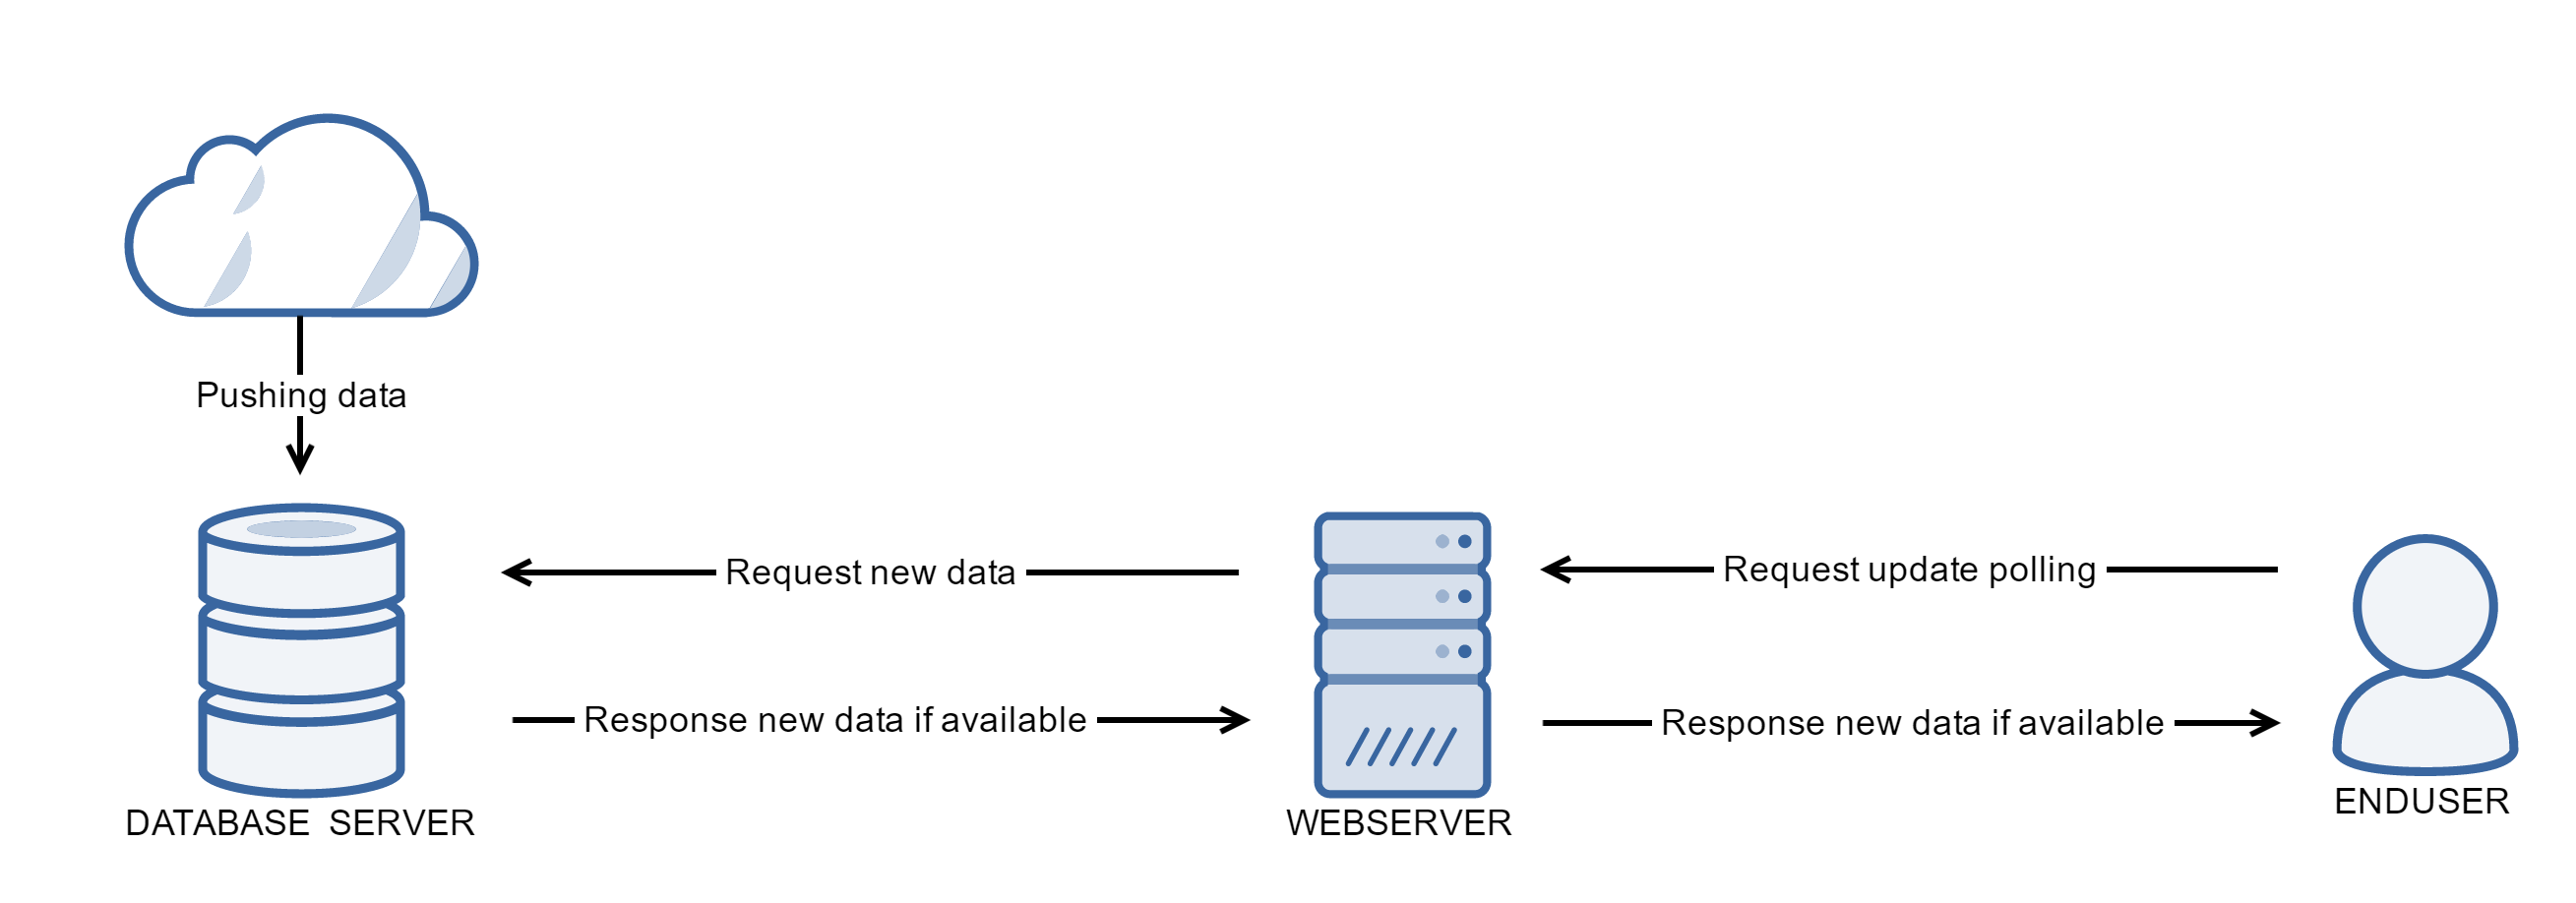
\includegraphics[width=1.0\textwidth]{polling}
	\caption[Mô hình tương tác polling]{Mô hình tương tác polling}
	\label{fig: polling}
\end{figure}
Phương pháp này dễ hiện thực và áp dụng, tuy nhiên sẽ mắc nhược điểm là tốn nhiều gói tin request vô dụng làm giảm hiệu năng hệ thống, và không đáp ứng tính realtime nếu như chu kì gửi request dài.



Vì hiện tại nhóm chúng tôi đang hướng tới hướng phát triển IoT, đòi hỏi yêu cầu về tính realtime cũng như tối ưu hóa hệ thống. Và để đáp ứng yêu cầu đó, nhóm đã tìm tới giải pháp giữ socket kết nối từ \textbf{Database} (RethinkDB) <-> \textbf{Server} (Chạy trên nền tảng Nodejs) <-> \textbf{Client} (web browser)

\begin{figure}[H]
	\centering    
	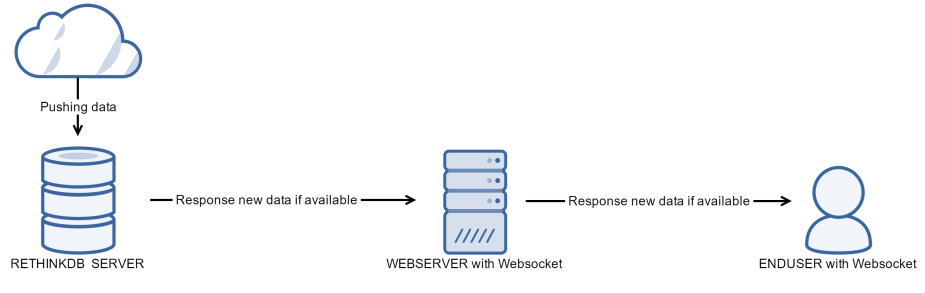
\includegraphics[width=1.0\textwidth]{realtime}
	\caption[Mô hình tương tác realtime dựa trên Socket]{Mô hình tương tác realtime dựa trên Socket}
	\label{fig: realtime}
\end{figure}

Như hình \ref{fig: realtime}, mô hình hoạt động đơn giản hơn rất nhiều, giảm bớt số lượng request không đáng có và đảm bảo tính realtime cho hệ thống.

Một điểm mạnh ở mô hình này nữa là có thể phát triển nhiều server hoặc ứng dụng di động sử dụng chung một hệ quản lý cơ sở dữ liệu nhưng vẫn đảm bảo sự đồng bộ dữ liệu cập nhật tới enduser theo thời gian thực.
\begin{figure}[H]
	\centering    
	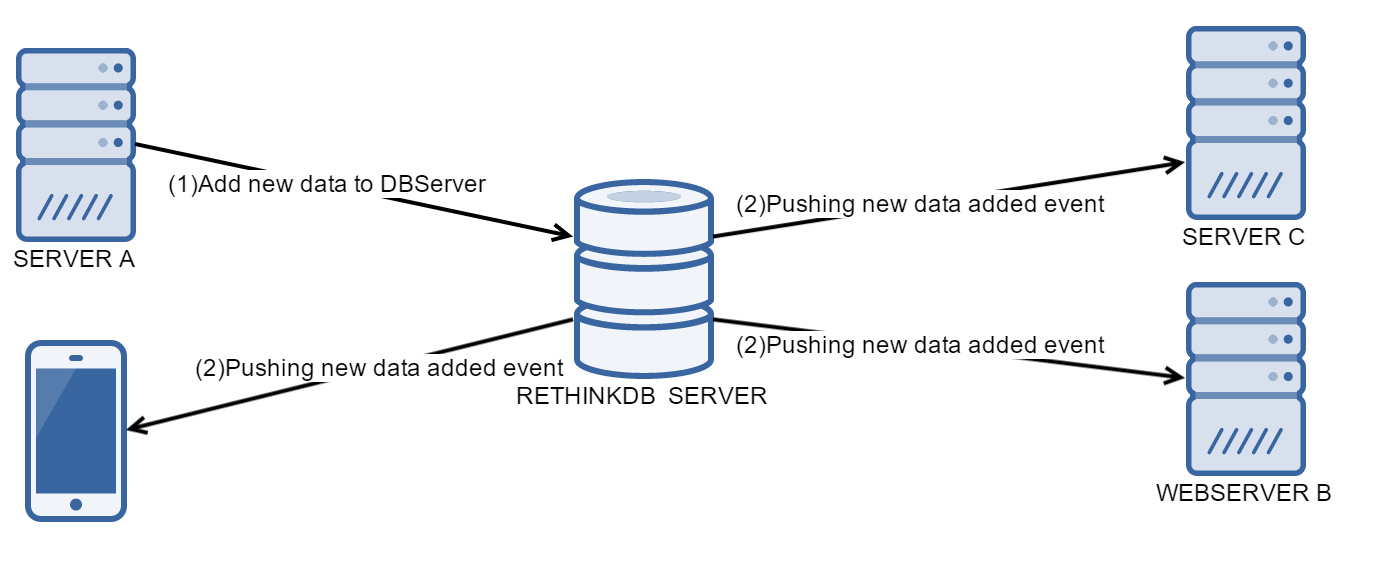
\includegraphics[width=1.0\textwidth]{multiserver}
	\caption[Mô hình tương tác cập nhật nhiều Server]{Mô hình tương tác cập nhật nhiều Server}
	\label{fig: multiserver}
\end{figure}






\newpage
\subsection{Mô hình ứng dụng trình bày dữ liệu}
\subsubsection*{Chức năng Web Server}
Đối với người dùng:
\begin{itemize}
\item[•] Cung cấp cho người dùng thông tin về nơi chứa node cảm biến.
\item[•] Người dùng có thể xem biểu đồ dữ liệu thông số môi trường tại vị trí tương ứng với node cảm biến đã được thiết lập.
\item[•] Xem được tình trạng và biểu đồ thống kê của các node cảm biến đang hoạt động.
\item[•] Gửi phản thông tin phản hồi về cho người quản lý thông qua email.
\item[•] Cung cấp thông tin lịch sử các hoạt động sử dung API, giúp cho bên thứ 3 có thể dễ dàng phát triển.
\end{itemize}

Đối với người quản lý:
\begin{itemize}
\item[•] Bao gồm tất cả chức năng của người dùng bình thường.
\item[•] Quản lý chỉnh sửa thông tin các node cảm biến: thêm, xóa, cập nhật, thay đổi.
\end{itemize}

\subsubsection*{Biểu đồ High level Usecase của Web Server}

\begin{figure}[H]
\centering    
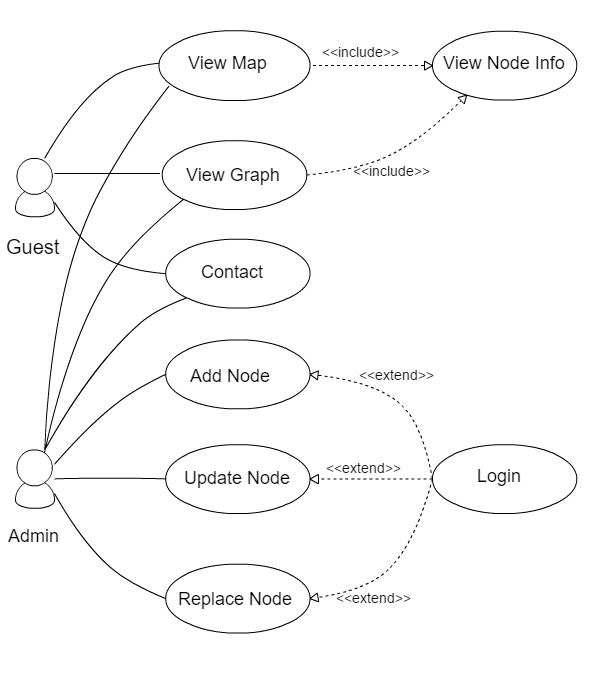
\includegraphics[width=0.7\textwidth]{usecase_diagram}
\caption[Biểu đồ High level Usecase]{Biểu đồ High level Usecase }
\label{fig:usecase_diagram}
\end{figure}

Mô tả giản đồ Usecase

\begin{table}[]
\centering
\caption{Bảng mô tả giản đồ Usecase của Web Server}
\label{my-label}
\begin{tabular}{|l|l|l|}
\hline
STT & Tên            & Miêu tả                                                                                            \\ \hline
1   & View map       & Người dùng thấy được các node đang chạy trên google maps                                           \\ \hline
2   & View Node Info & Thông tin tương ứng của Node( Lat, Lng, Phone)                                                     \\ \hline
3   & View Graph     & \begin{tabular}[c]{@{}l@{}}Đồ thị hoạt động của Node(các số liệu đo được theo\\ ngày)\end{tabular} \\ \hline
4   & Contact        & Phản hồi ý kiến người dùng qua Gmail                                                               \\ \hline
5   & Add Node       & Thêm mới Node vào hoạt động                                                                        \\ \hline
6   & Update Node    & Thay đổi thông tin của Node( Lat, Lng, Phone)                                                      \\ \hline
7   & Replace Node   & Thay đổi 1 Node xảy ra sự cố bằng 1 Node khác                                                      \\ \hline
\end{tabular}
\end{table}




%%%%%%%%%%%%%%%%%%%%%%%%%%%%%%%%%%%%%%%%%%%%%%%%%%%%%%%%%%%%%%%%%%%%%%%%%%
% 				VẼ MẤY CÁI D.	Acitivity diagram VÀO ĐÂY %%%%%%%%%%%%%%%%%
%%%%%%%%%%%%%%%%%%%%%%%%%%%%%%%%%%%%%%%%%%%%%%%%%%%%%%%%%%%%%%%%%%%%%%%%%%%%%




\subsubsection*{Chức năng Ứng dụng di động}
Hiện thị thông tin các node cảm biến đang hoạt động qua màn hình chính, và biểu đồ dữ liệu của từng node cảm biến theo từng ngày, thêm sự kết nối với web browser tạo sự thuận tiện cho việc theo dõi, hiện thị đồ thị (2 kiểu đồ thị là line chart và bar chart).
\subsubsection*{Biểu đồ High level Usecase của ứng dụng di động}

\begin{figure}[H]
\centering    
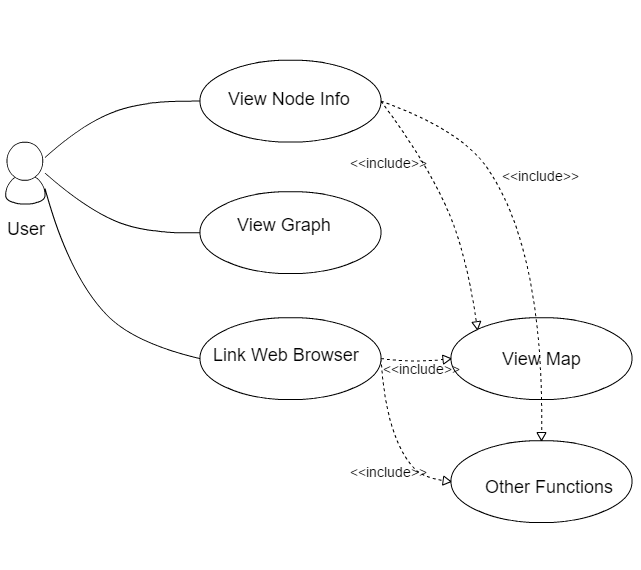
\includegraphics[width=0.7\textwidth]{app_usecase}
\caption[Giản đồ High level Usecase của ứng dụng di động]{Giản đồ High level Usecase của ứng dụng di động}
\label{fig:app_usecase}
\end{figure}

Mô tả Usecase

\begin{table}[H]
\centering
\caption{Bảng mô tả giản đồ Usecase của ứng dụng di động}
\label{table:usecase_mobile}
\begin{tabular}{|l|l|l|}
\hline
STT & Tên Use-case     & Mô tả                                                            \\ \hline
1   & View Node Info   & Thông tin của Node( Lat, lng, Phone, ID)                         \\ \hline
2   & View Graph       & 2 dạng đồ thị theo ngày (line chart, bar chart của các thông số) \\ \hline
3   & Link web browser & Liên kết tới web browser                                         \\ \hline
4   & View Map         & Hiện thị Google Map và vị trí các Node                           \\ \hline
5   & Other Functions  & Các chức năng của web browser                                    \\ \hline
\end{tabular}
\end{table}













\subsection{Các ràng buộc của hệ thống}
Cũng như các dự án IoT quy mô rộng khác, đề tài cũng yêu cầu nhiều đặc tính ràng buộc như:  
\subsubsection*{Tính đáp ứng thời gian thực:}Để giải quyết tình trạng giao thông hiện thời và trong thời gian gần, ta cần phải có dữ liệu thời gian thực. Ta không thể sử dụng dữ liệu của nửa tiếng hoặc 1 giờ trước để vẽ nên bản đồ lưu thông hiện tại cũng như cách điều hướng giải quyết. Do đó, hệ thống cần phải có thời gian đáp ứng nhanh khi có yêu cầu dữ liệu khi được gọi. Để đạt được kết quả đó, ta cần phải có những phần cứng với thiết lập kết nối có khả năng đáp ứng nhanh, cùng với khả năng hoạt động ổn định liên tục trong thời gian dài để cung cấp dữ liệu liên tục và liền mạch.


\subsubsection*{Toàn ven dữ liệu (Data Integrity):} Mục đích chính của dự án là thu thập dữ liệu và từ đó phát triển ứng dụng. Vì thế tính toàn vẹn dữ liệu đóng vai trò quan trọng. Dữ liệu thu thập cần phải đáp ứng đủ các yếu tố: tin cậy, chính xác và đầy đủ. Ta cần phải có đủ dữ liệu thì mới có thể đủ dữ kiện để giải quyết bài toán. Ta không thể giải quyết khi chỉ có được dữ liệu một đoạn đường, 1 thời gian ngắn mà đòi hỏi phải có dữ liệu của một khu vực đủ lớn và tương quan với nhau. Bên cạnh đó cần phải có tính chính xác dữ liệu và đòi hỏi sự ổn định của lượng dữ liệu đó qua yếu tố độ tin cậy. 
\begin{center}
\begin{figure}[htp]
\centering    
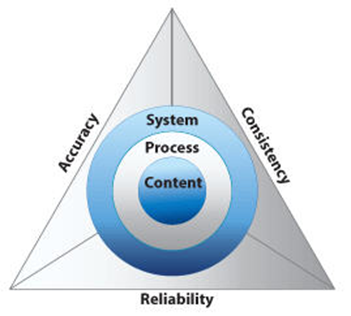
\includegraphics[width=3in]{toanvendulieu}
\caption[Toàn ven dữ liệu]{Toàn ven dữ liệu}
\label{fig:toanvendulieu}
\end{figure}
\end{center}

\subsubsection*{Đồng bộ hóa:} Hệ thống giám sát môi trường có nhiều thiết thiết bị khác nhau, nhiều phương pháp và cách thức truyền dữ liệu khác nhau. Do đó ta cần phải có sự chuẩn hóa các giao thức giao tiếp, đồng bộ các gói dữ liệu. Tuy nhiên điều này sẽ dẫn đến vấn nạn được đề cập ở mục sau.

\subsubsection*{Tính bảo mật:} Vấn đề bảo mật và an toàn dữ liệu hiện tại vẫn là một trong những khó khăn mà hệ thống IoT đang mắc phải. Vì hệ thống IoT đòi hỏi cần phải có giao thức kết nối giữa các thiết bị phải được chuẩn hóa và động bộ, cũng như tối giản kích thước gói tin để tối ưu trong việc truyền dữ liệu giữa các thiết bị, do đó gói tin truyền đi có thiết lập cấu trúc đơn giản và hệ thống dễ bị thâm nhập. Điều này sẽ dẫn đến hệ thống có thể bị đánh cắp dữ liệu, và thậm chí mất quyền kiểm soát toàn bộ hệ thống bởi vì tất cả đều được kết nối với nhau. Vậy nên cần phải cân nhắc trade-off giữa hiệu năng hệ thống và tính bảo mật.
\begin{center}
\begin{figure}[htp]
\centering    
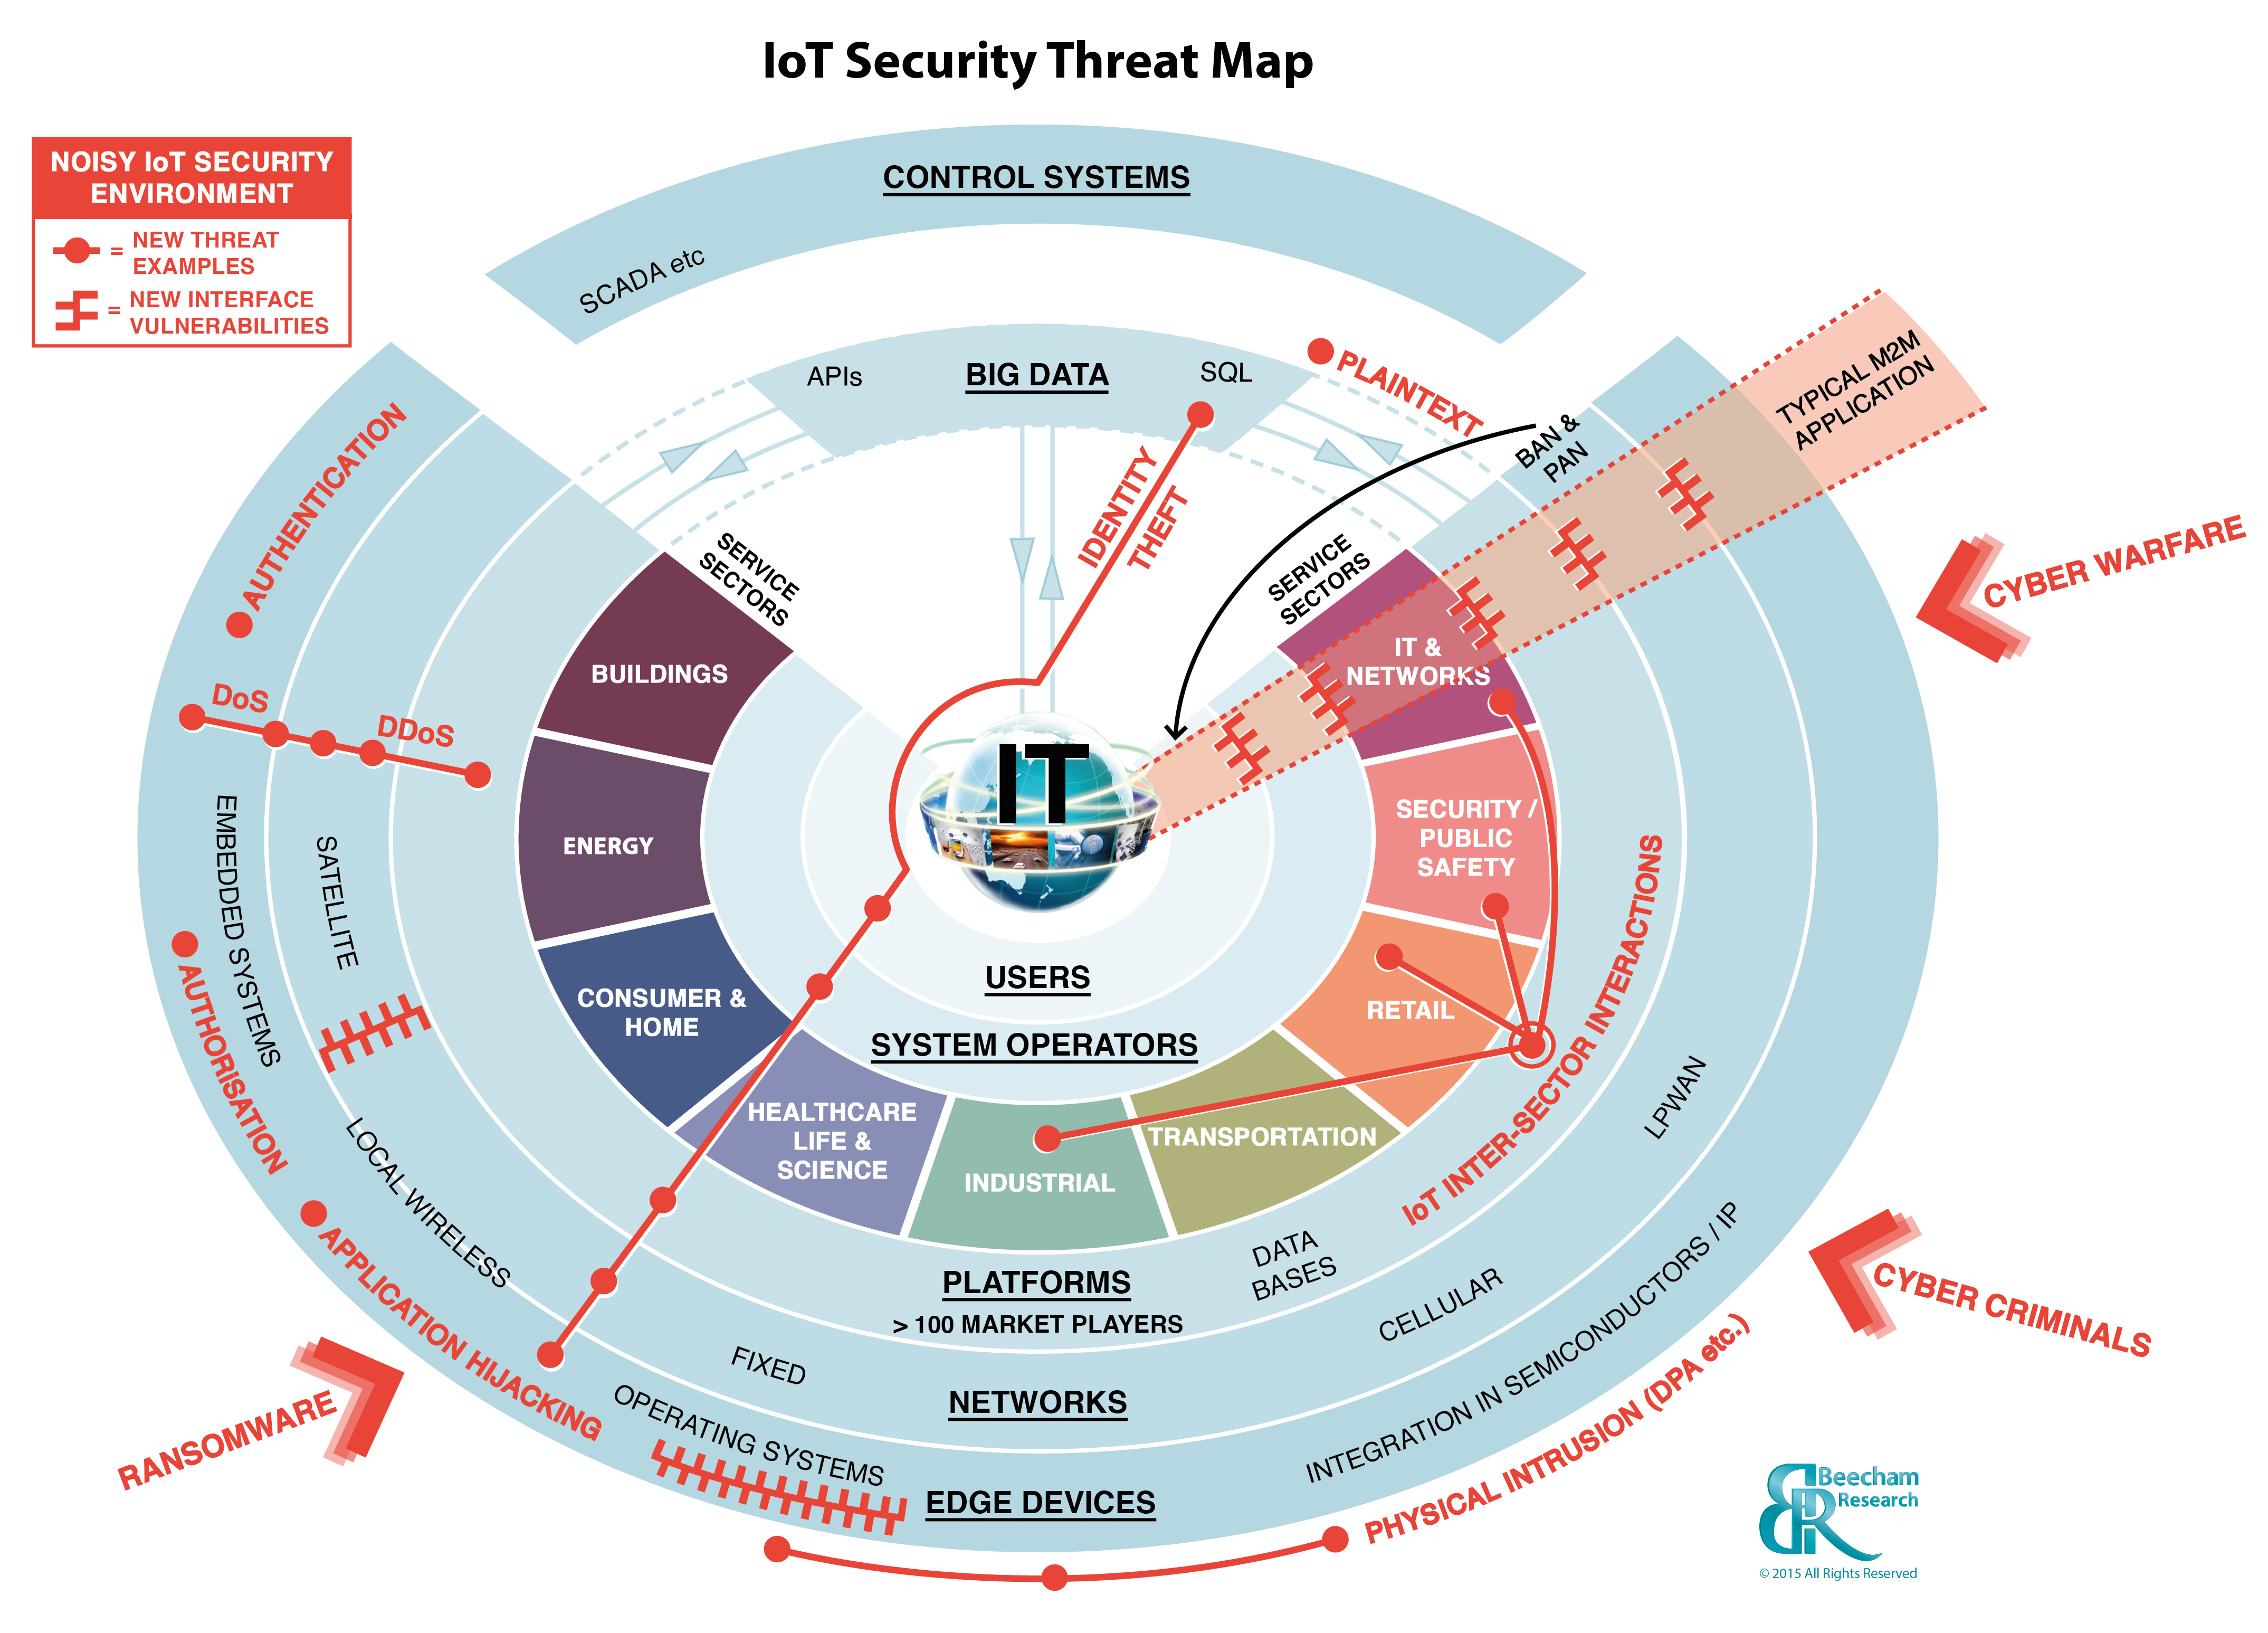
\includegraphics[width=5in]{virusiot}
\caption[Tính bảo mật]{Tính bảo mật}
\label{fig:virusiot}
\end{figure}
\end{center}
Các mối nguy hại chính ảnh hưởng trực tiếp tới hệ thống IoT như: DDoS, Ransomware, Cyber Criminals và Cyber Warfare. 











\section{Hiện thực Node cảm biến}
\subsection{Các node cảm biến thu thập dữ liệu}
Lorem ipsum dolor sit amet, consectetur adipiscing elit, sed do eiusmod tempor incididunt ut labore et dolore magna aliqua. Ut enim ad minim veniam, quis nostrud exercitation ullamco laboris nisi ut aliquip ex ea commodo consequat. Duis aute irure dolor in reprehenderit in voluptate velit esse cillum dolore eu fugiat nulla pariatur. Excepteur sint occaecat cupidatat non proident, sunt in culpa qui officia deserunt mollit anim id est laborum
\subsection{Ứng dụng theo dõi dữ liệu và đánh giá}
Lorem ipsum dolor sit amet, consectetur adipiscing elit, sed do eiusmod tempor incididunt ut labore et dolore magna aliqua. Ut enim ad minim veniam, quis nostrud exercitation ullamco laboris nisi ut aliquip ex ea commodo consequat. Duis aute irure dolor in reprehenderit in voluptate velit esse cillum dolore eu fugiat nulla pariatur. Excepteur sint occaecat cupidatat non proident, sunt in culpa qui officia deserunt mollit anim id est laborum
\section{Hệ thống Server lưu trữ dữ liệu và cung cấp API}
Lorem ipsum dolor sit amet, consectetur adipiscing elit, sed do eiusmod tempor incididunt ut labore et dolore magna aliqua. Ut enim ad minim veniam, quis nostrud exercitation ullamco laboris nisi ut aliquip ex ea commodo consequat. Duis aute irure dolor in reprehenderit in voluptate velit esse cillum dolore eu fugiat nulla pariatur. Excepteur sint occaecat cupidatat non proident, sunt in culpa qui officia deserunt mollit anim id est laborum
\subsection{Cấu trúc tổ chức tập tin}
\subsubsection*{Các thư mục và chức năng}
\begin{figure}[H]
	\centering    
	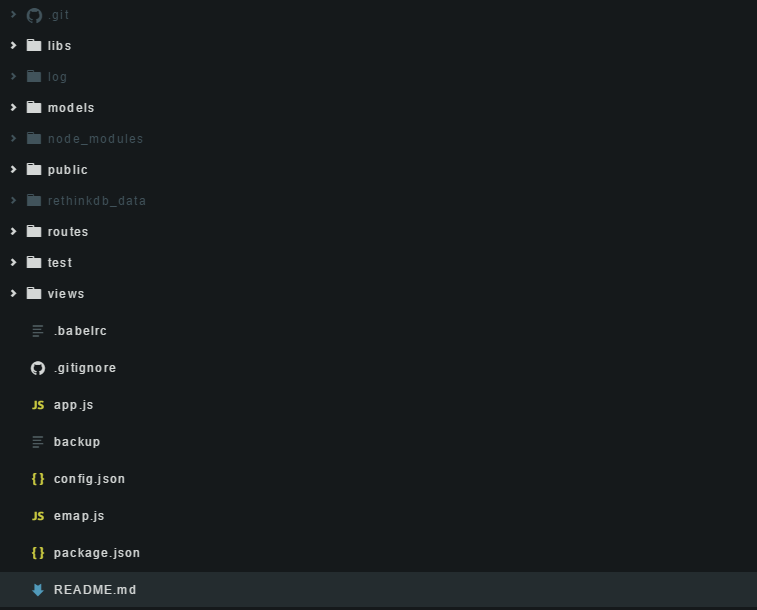
\includegraphics[width=1.0\textwidth]{tree}
	\caption[Mô hình hoạt động Nodejs]{Mô hình hoạt động Nodejs}
	\label{fig: tree}
\end{figure}
Như hình \ref{fig: tree}, chúng ta có những thư mục được làm việc trực tiếp:

• libs: chứa các hàm function hỗ trợ về xác thực và log.

• models: thư mục này bao gồm các mô hình quản lý cơ sở dữ liệu.

• routes: điều khiển và điều hướng theo các url.

• log: chứa các file ghi lại log trong quá trình hoạt động.

• views: là bộ mặt của web server, giúp người dùng có thể tương tác được với server qua web browser, bao gồm các file giao diện như html, ejs...   


\subsubsection*{Các file khởi tạo và cấu hình Server}

\textbf{Các file khởi tạo này bao gồm:}

• emap.js: file có chức năng đọc file cấu hình và khởi tạo kết nối server.
\begin{lstlisting}[caption=emap.js]
...
server.on('listening', onListening); // open for listening
function onListening() {
	var addr = server.address();
	var bind = typeof addr === 'string' ?
	'pipe' + addr :
	'port' + addr.port;
	debug('Listening on ' + bind);
	console.log('Listening on ' + bind);
};
...
\end{lstlisting}

• app.js: là file điều khiển và thiết lập các chức năng, khai báo các modules chính được sử dụng. Bên cạnh đó, còn có chức năng gán điều hướng tới các file trong thư mục route
\begin{lstlisting}[caption=app.js]
...
// initial server
app.use(passport.initialize());
app.use(passport.session());
app.set('views', path.join(\_\_dirname, 'views'));
app.engine('ejs', engine);
...
// control route
app.use(logger('dev'));
app.use('/log', express.static(path.join(__dirname, 'log')));
app.use(express.static(path.join(__dirname, 'public')));
app.use('/log', serveIndex('./log'));
app.use('/', routes);
app.use('/user', user);
app.use('/node', node);
app.use('/auth', auth);
...
\end{lstlisting}

\textbf{Các file cấu hình này bao gồm:}

• package.json: khai báo các thông tin cơ bản về project và các modules được sử dụng.
\begin{lstlisting}[caption=package.json]
{
	"name": "emap-server",
	"version": "1.0.0",
	"description": "This is serverside part of IoT project",
	"main": "emap.js",
	"author": "Cuong, Tung and Ny",
	"license": "ISC",
	"homepage": "www.codingyourfuture.com",
	"dependencies": {			// dependancies modules
		"angular-chart.js": "^1.0.3",
		"asyncawait": "^1.0.6",
		"babel": "^6.5.2",
		"ejs": "^2.5.2",
		...
		"rethinkdb": "^2.3.3",
		"serve-index": "^1.8.0",
		"socket.io": "^1.5.0",
	}
}
\end{lstlisting}
• config.json: khai báo các thông số cấu hình được sử dụng. Tại đây ta cấu hình thông số kết nối tới RethinkDB và port ứng dụng server nodejs.
\begin{lstlisting}[caption=config.json]
{
	"app":{
		"port": "8888"
	},
	"rethinkdb":{
		"host": "localhost",
		"port" : "28015",
		"db": "emap",
		"address":"localhost:28015",
		"tableList":["nodeData"]
	}
}

\end{lstlisting}


%% Thiết kế API

\subsection{Thiết kế API}

Mục tiêu đề tài không chỉ thu thập và phân tích mà còn chia sẻ dữ liệu. Để làm được điều đó thì cần phải có API cung cấp cho những nhà phát triển thứ 3, có thể dùng API được cung cấp để sử dụng dữ liệu để phát triển. Bởi vì vậy hệ thống có xây dựng hệ thống API mở.

\subsubsection*{API List}
Ở bảng \ref{table: apilist}

\begin{table}[H]
	\centering
	\caption{Bảng API tương tác với dữ liệu về các node}
	\begin{tabular}{|l|l|l|l|}
		\hline
		Method & URL            & Miêu tả         & Yêu cầu xác thực người dùng        \\ \hline
		POST   & /node/initnew       & Khởi tạo node mới                & Có           \\ \hline
		POST   & /node/updatenode     & Cập nhật thông tin node & Có \\ \hline
		POST   & /node/replacenode       & Thay thế node  & Có       \\ \hline
		GET   & /node/pushdata & Push dữ liệu               &         Không                \\ \hline
		GET   & /node/getdata    & Get dữ liệu thu thập của node         &  Không      \\ \hline
		GET   & /node/getinfo   & Get thông tin của node & Không  \\ \hline
	\end{tabular}
	\label{table: apilist}
\end{table}

/node/initnew
/node/pushdata
/node/updatenode
/node/replacenode
/node/getdata
/node/getinfo



\subsection{Hiện thực Server}
\subsection{Xây dựng Web Server}





\subsection{Hiện thực giao diện}

Sử dụng framework express của Nodejs và HTML để xây dựng frontend


\subsubsection*{Giao diện chính của Web Server}
Phần này chứa các nút menu chức năng cùng với google map để theo dõi vị trí hoạt động của các cảm biến.
\begin{center}
\begin{figure}[htp]
\centering    
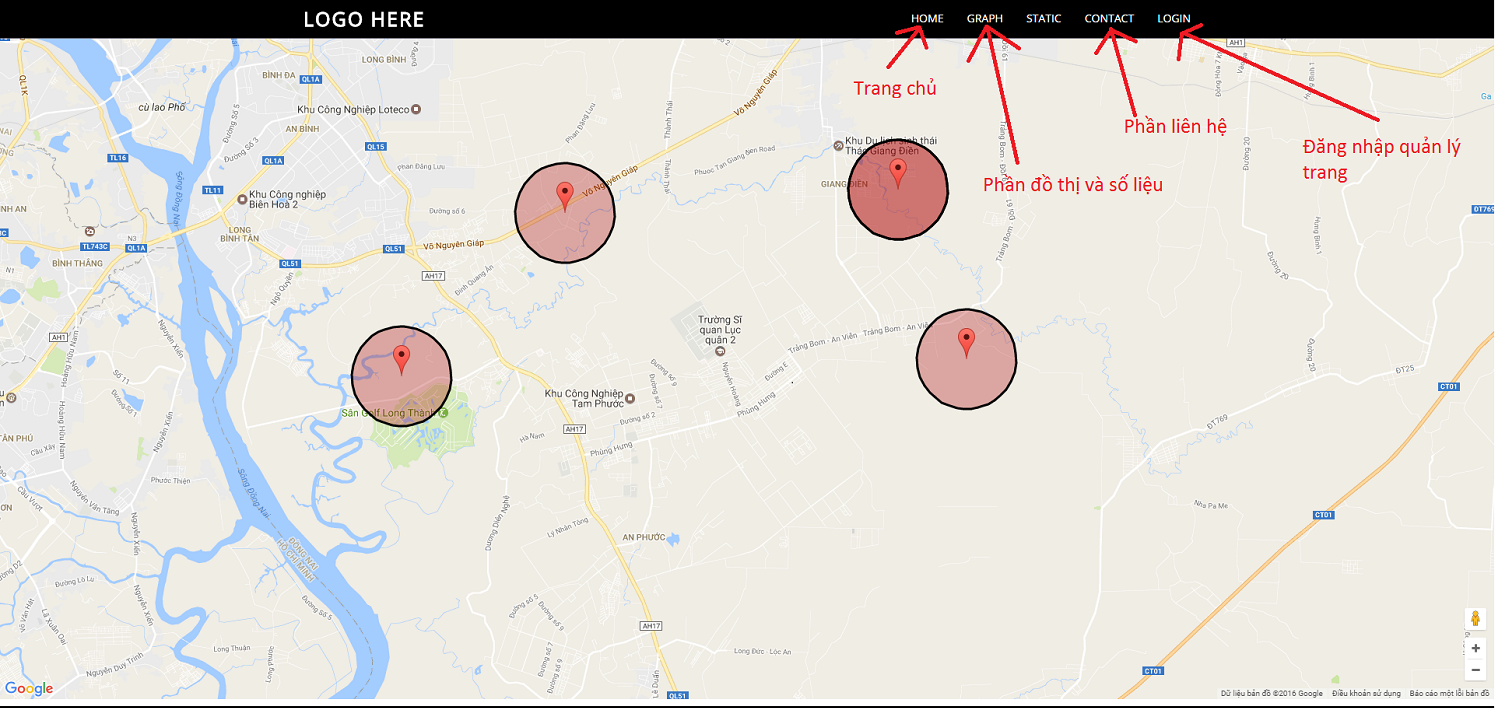
\includegraphics[width=1\textwidth]{webserver}
\caption[Giao diện chính của Web Server]{Giao diện chính của Web Server}
\label{fig:webserver}
\end{figure}
\end{center}

\subsubsection*{Giao diện đồ thị dữ liệu}
Là nơi hiện thị biểu đồ của các thông số cũng như thông tin tương ứng của các cảm biến.
\begin{center}
\begin{figure}[htp]
\centering    
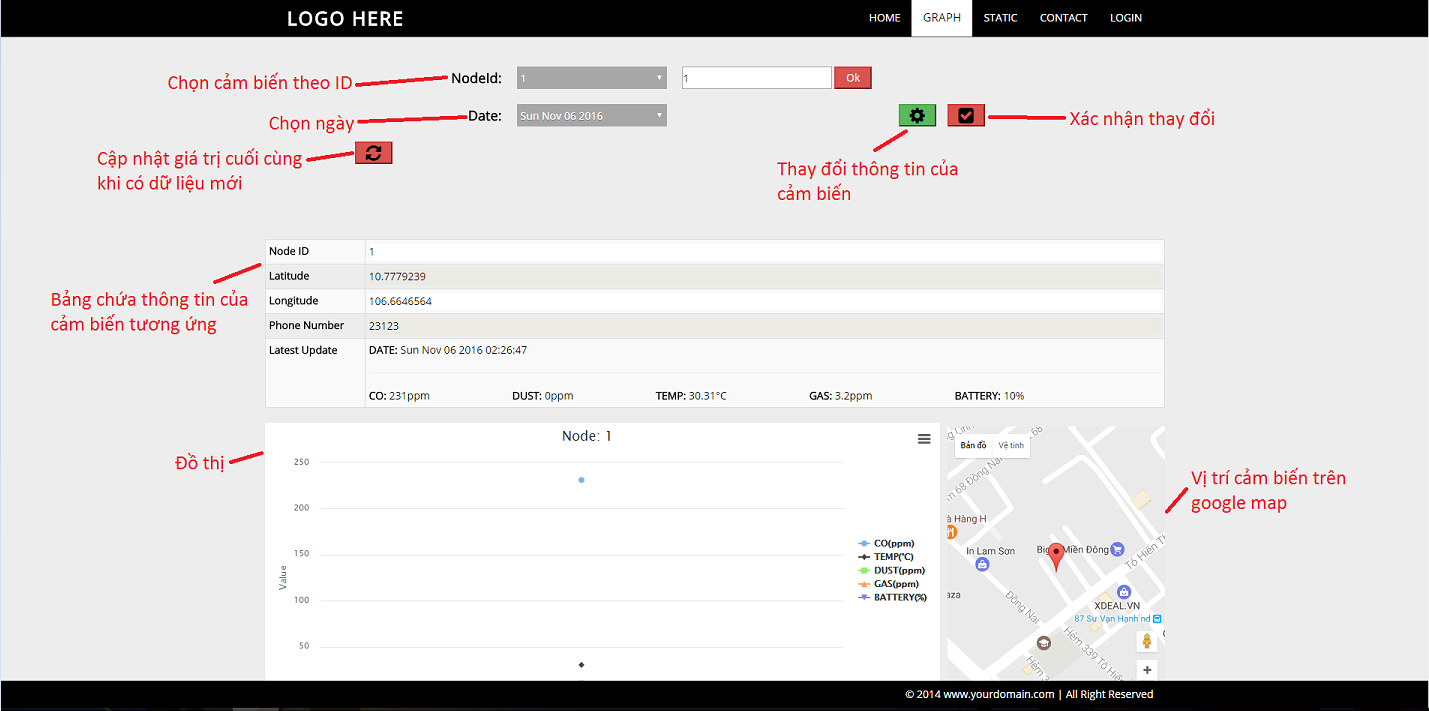
\includegraphics[width=1\textwidth]{web_graph}
\caption[Giao diện đồ thị dữ liệu]{Giao diện đồ thị dữ liệu}
\label{fig:web_graph}
\end{figure}
\end{center}



\subsubsection*{Giao diện nhận feedback từ người dùng qua email}
Tương tác giữa người dùng với người quản lý server. Nội dung được gửi thông qua gmail.
\begin{center}
\begin{figure}[htp]
\centering    
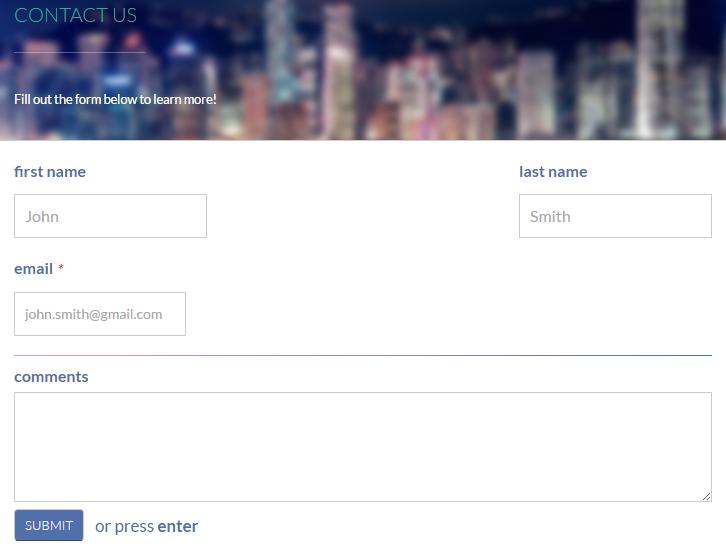
\includegraphics[width=1\textwidth]{web_email}
\caption[Giao diện nhận feedback người dùng]{Giao diện nhận feedback người dùng}
\label{fig:web_email}
\end{figure}
\end{center}

\subsubsection*{Giao diện dành cho người quản lý}
Khu vực này dành cho người quản lý truy cập nhầm mục đích chỉnh sửa, thay thế các node cảm biến.
\begin{center}
\begin{figure}[htp]
\centering    
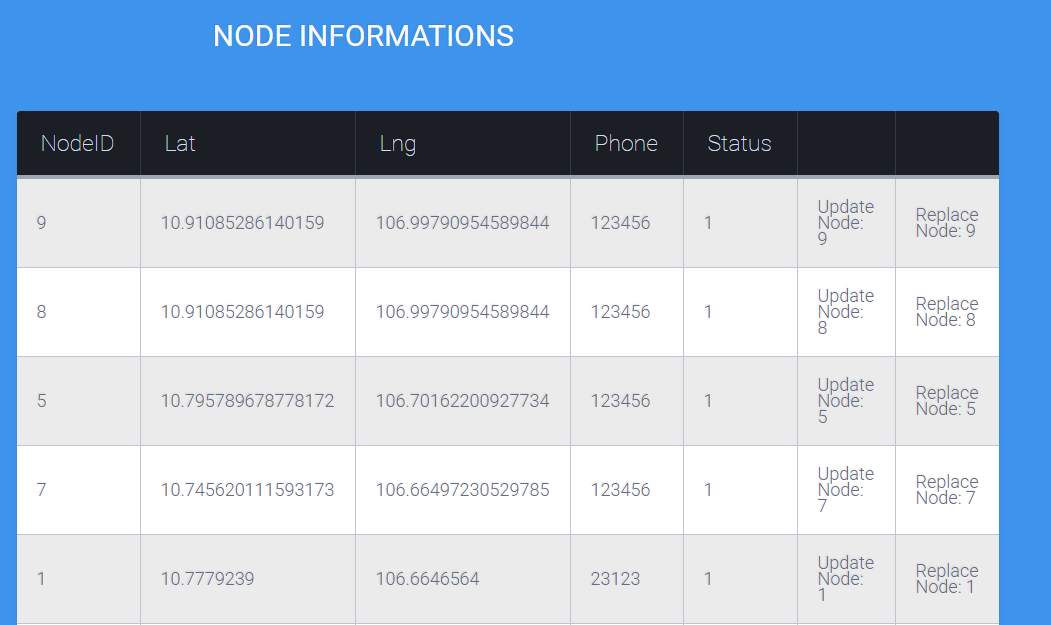
\includegraphics[width=1\textwidth]{web_nodeinfo}
\caption[Giao diện quản lý các node cảm biến]{Giao diện quản lý các node cảm biến}
\label{fig:web_nodeinfo}
\end{figure}
\end{center}





\section{Ứng dụng thiết bị di động}




\subsection{Hiện thực giao diện và chức năng}
\subsubsection*{Giao diện chính ứng dụng di động}
Tại giao diện chính của ứng dụng di động người dùng có thể xem được danh sách thông tin chi tiết của các node cảm biến có trong hệ thống.
\begin{center}
\begin{figure}[htp]
\centering    
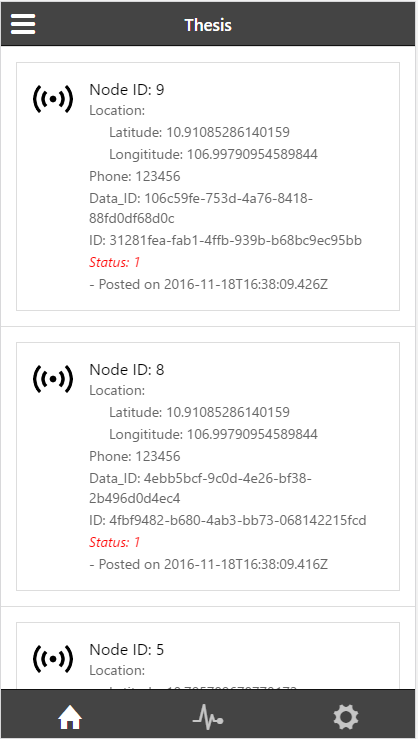
\includegraphics[width=0.4\textwidth]{app_main}
\caption[Giao diện chính ứng dụng di động]{Giao diện chính ứng dụng di động}
\label{fig:app_main}
\end{figure}
\end{center}


\subsubsection*{Giao diện xem dữ liệu trên ứng dụng di động}
Giao diện này cho phép người dùng theo dõi được dữ liệu của từng node cảm biến theo 2 loại biểu đồ như Hình \ref{fig:app_graph} thể hiện.
\begin{center}
\begin{figure}[htp]
\centering    
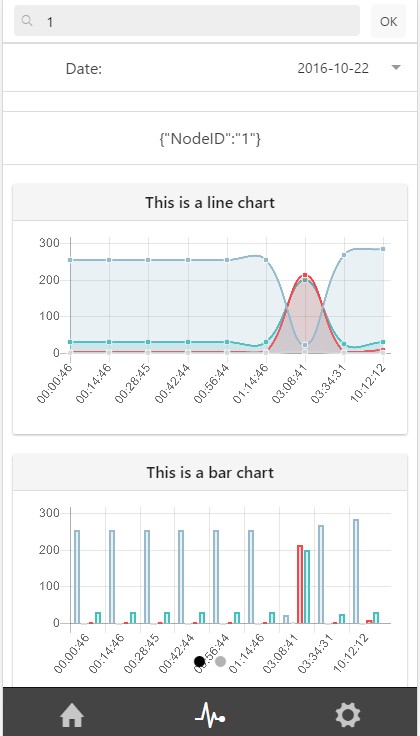
\includegraphics[width=0.4\textwidth]{app_graph}
\caption[Giao diện xem dữ liệu trên ứng dụng di động]{Giao diện xem dữ liệu trên ứng dụng di động}
\label{fig:app_graph}
\end{figure}
\end{center}


